\chapter{Images of the experiments}

\section{Mobile application screenshots}

\clearpage
\newpage

\section{Training procedure experiments}
Next we demonstrate most of the experiments as collations of training and test images, as well as plots of training losses and plots of validation metrics. Images encased with a gray border are \textit{synthesized}, the border-less images are ground truth. Each column of the images has a colored mark at the bottom. It represents a corresponding line color on the plots for the given experiment. The legends of the plots contain a short description of the experimental setup and adjustments. To shorten the descriptions, we use a notation like $\Omega=$ to show that any other usage of $\Omega$ on the same plot uses or extends from this experiment. 

To keep this section compact, we demonstrate plots of LPIPS, L1, MS-SSIM, and adversarial losses. A single plot of the adversarial loss will combine two lines: generator's loss (solid line) is accuracy of the discriminator on the synthesized images, the discriminator's loss (translucent line with colored dots) is accuracy of the discriminator on the real images. The former should decrease, indicating that the generator produces plausible images, and the latter should increase, indicating that the discriminator learns the realism of ground truth images.

As a minimal subset of training images, we show full-body and upper body frames with the most difficult poses available, frames from front and back, as well as a close-up shot of a face. The selected test frames contain:
\begin{itemize}
	\item Bottom of the shoes -- showing artifacts for the body parts that were unseen during training.
	\item A face close-up -- may lose similarity with the person's face due to overfitting.
	\item A top-down view, which may show overfitting to the frames in the training set, where the person bends forward, and a shadow is cast upon their upper body (see training images, first row). Even though the test pose is different, the overfitting triggers the same shadow to appear on the synthesized image.
	\item An upper-body, to compare clarity of T-shirt ornaments, which may be lose due to possible misalignment of the ground truth images and the body model \cite{dnn:smplx19}. Thus, the pixels of the neural texture may fit different locations on the body.
	\item A front full-body view, to compare overall body quality.
\end{itemize}

\newcounter{experiments-group}
\setcounter{experiments-group}{1}

\setkeys{Gin}{draft}
\clearpage
\newpage
\arabic{experiments-group}. \alert{Experiments on neural texture's MIP-maps (no Omega definition for test plot)}
\stepcounter{experiments-group}
%\begin{adjustwidth}{-20em}{-8em}

% convert -strip -interlace Plane -quality 95% -adaptive-resize 85% TEST_05_54_r1\@vA01_41\@vA01_41_learnmips\@vA01_41_nomips.png out2.jpg
\begin{figure}[!h]
	\makebox[\textwidth]{\makebox[1.1\textwidth]{
	\begin{minipage}[b]{.59\textwidth}
		\centering%
		\setlength\abovedisplayskip{0pt}%
		\centerline{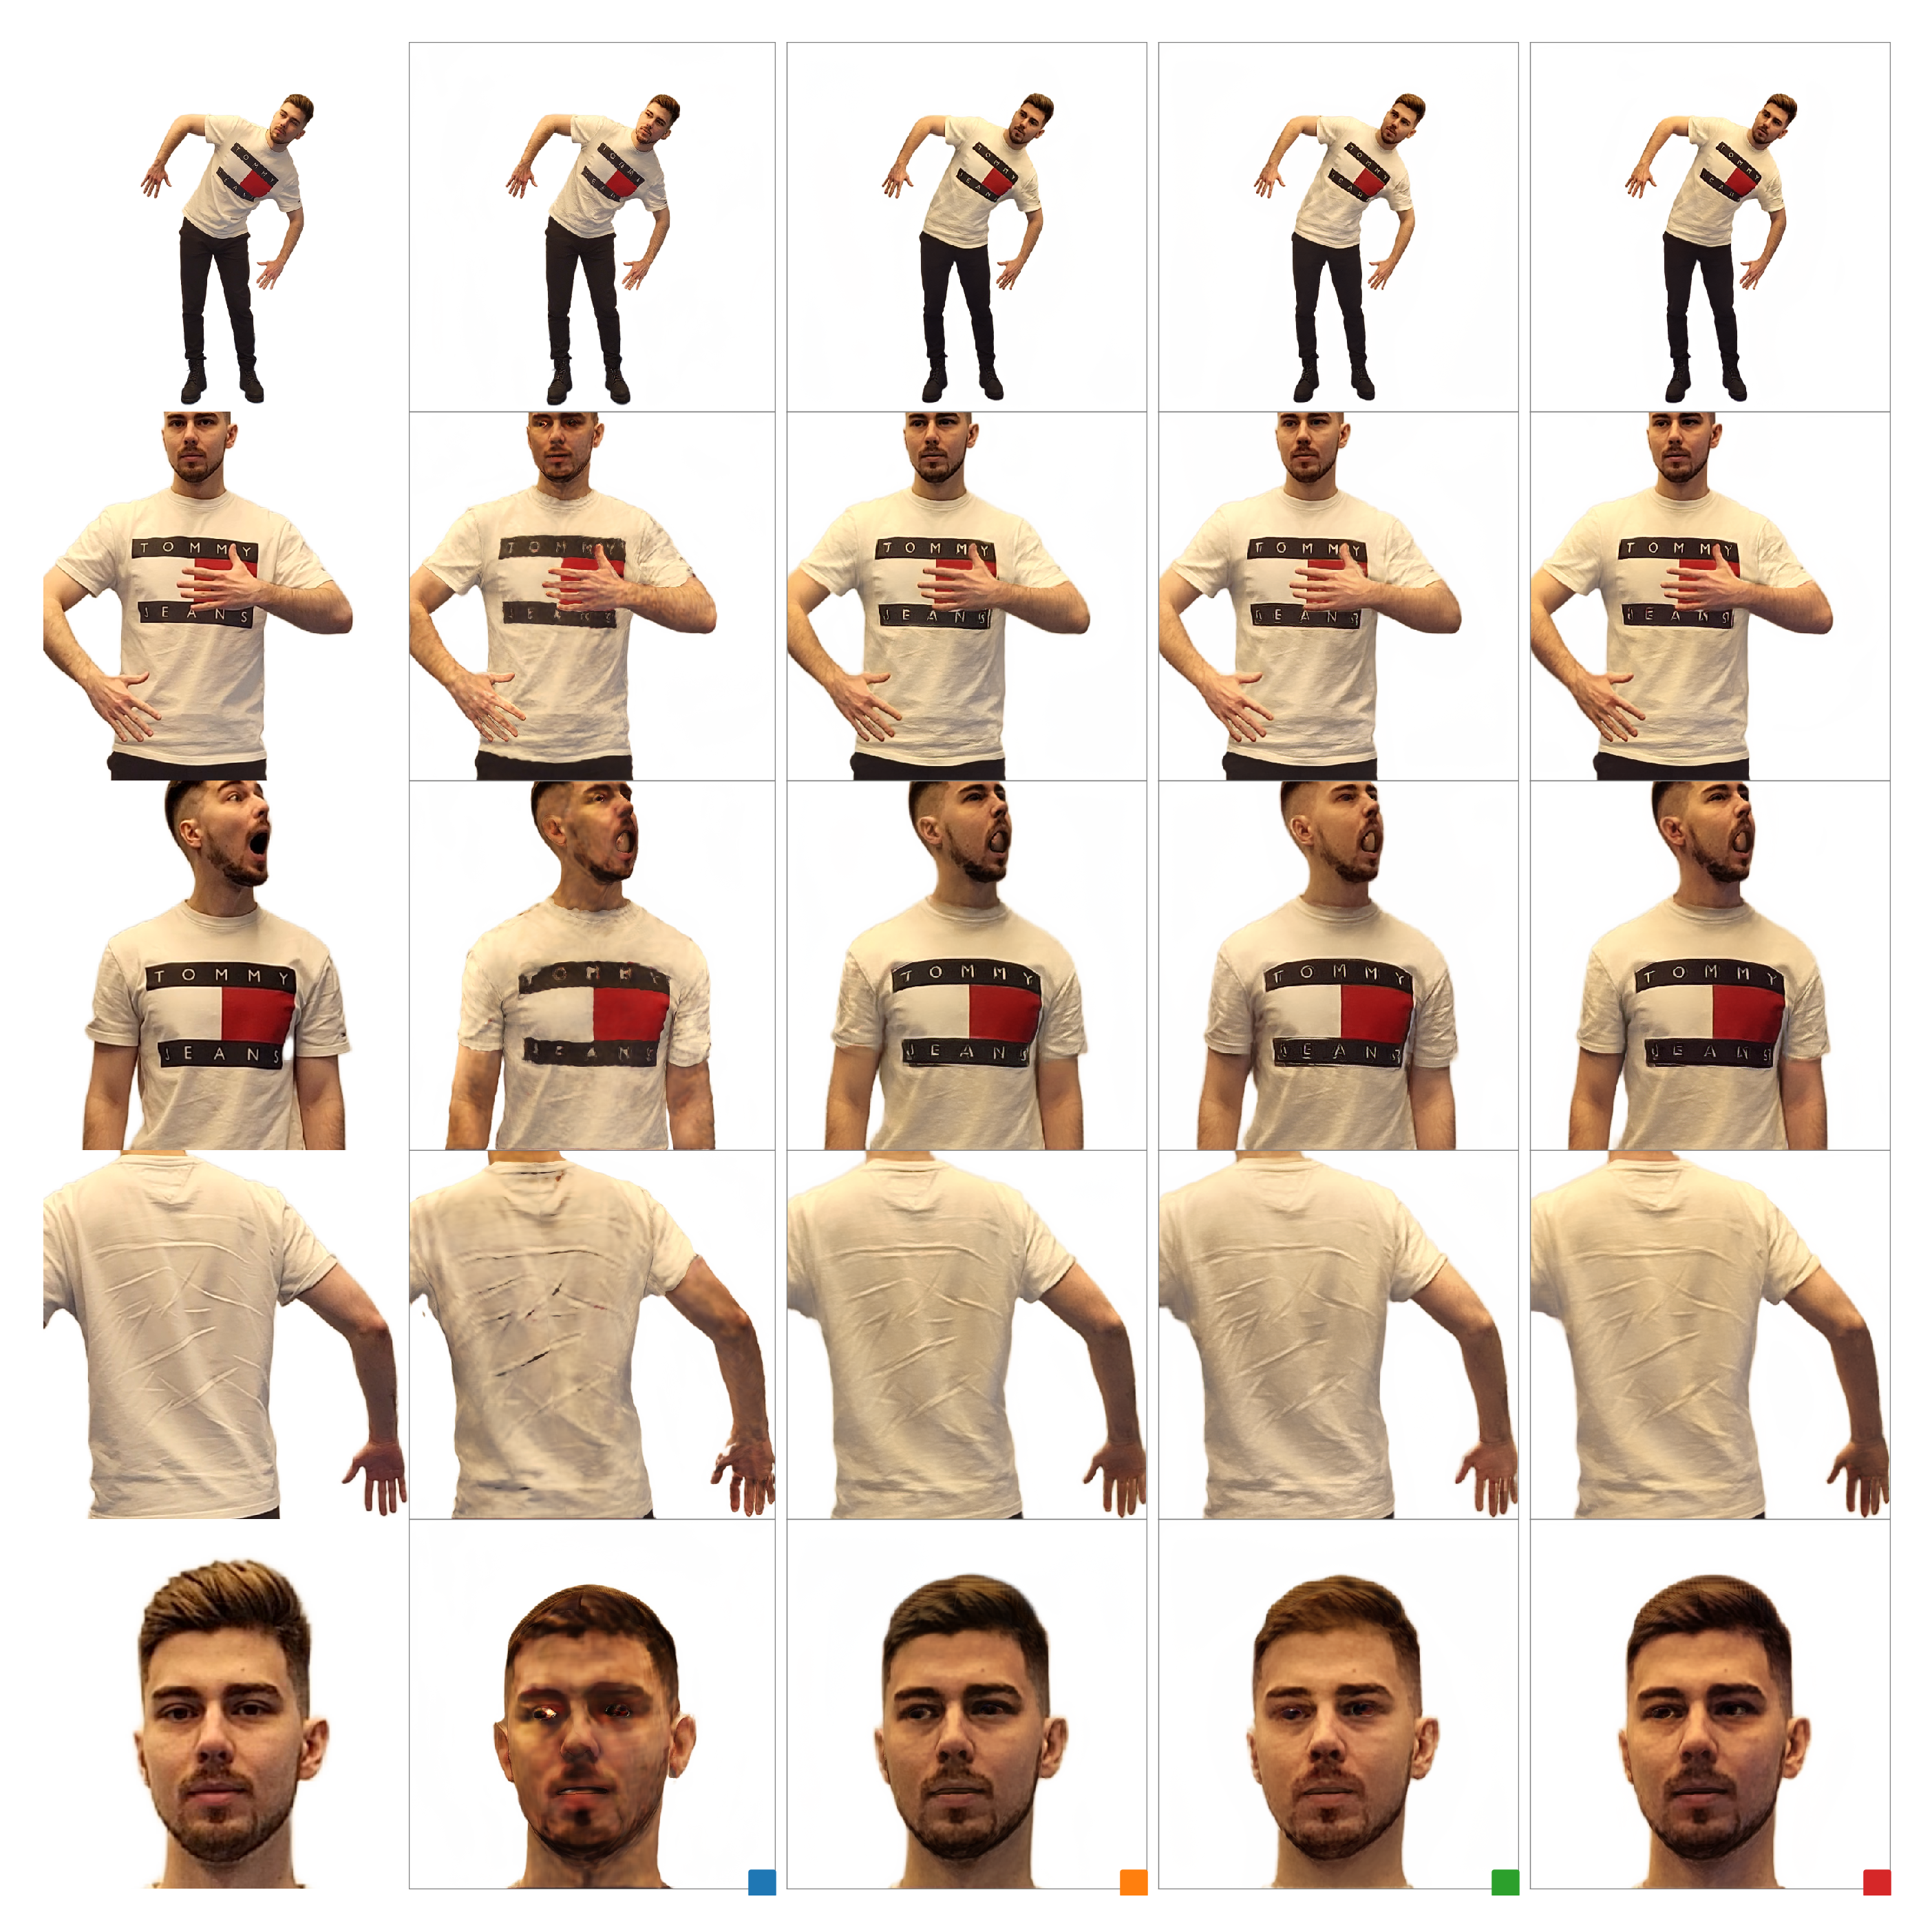
\includegraphics[width=1.0\textwidth]{\imgfp/exp_train/TRAIN_05_54_r1@vA01_41@vA01_41_learnmips@vA01_41_nomips}}%
		\caption{Fit to ground truth}
		\setlength\belowdisplayskip{0pt}%
	\end{minipage}\hfill
	\begin{minipage}[b]{.50\textwidth}
		\centering%
		\setlength\abovedisplayskip{0pt}%
		\centerline{\includegraphics[width=1.0\textwidth]{\imgfp/exp_test/TEST_05_54_r1@vA01_41@vA01_41_learnmips@vA01_41_nomips}}%
		\caption{Test images}
		\setlength\belowdisplayskip{0pt}%
	\end{minipage}
	}}
	\centering%
	%\hspace{.1\textwidth}%
	\setlength\abovedisplayskip{0pt}%
	\centerline{\includegraphics[width=0.99\linewidth]{\imgfp/exp_train/train_plot_05_54_r1@vA01_41@vA01_41_learnmips@vA01_41_nomips}}%
	\hspace{.1\textwidth}
	\centerline{\includegraphics[width=0.99\linewidth]{\imgfp/exp_test/val_plot_05_54_r1@vA01_41@vA01_41_learnmips@vA01_41_nomips}}%
	\setlength\belowdisplayskip{0pt}%
	\caption{Training losses and validation metrics}
\end{figure}
%\end{adjustwidth}

\newpage


\setkeys{Gin}{draft=false}
